% !TeX root = ./main.tex
\documentclass[main]{subfiles}
\begin{document}
\chapter{Аксиомы отделимости}
\section{Аксиомы отделимости}\marginpar{23.05.22}
\begin{theorem}[$T_0$, акcиома Колмогорова]
    $\forall x, y \in X\ \exists U$ -- открытое, которое  содержит ровно одну из этих точек.
\end{theorem}
\begin{theorem}[$T_1$]
    $\forall x, y \in X\ \exists U_x$ -- открытое, т.ч. $x\in U_x, y \not\in U_x$.
\end{theorem}
\begin{theorem}[$T_2$, аксиома Хаусдорфа]
    $\forall x,y \in X\ \exists U_x, U_y$ -- открытые окрестности, т.ч. $U_x \cap U_y = \varnothing$
\end{theorem}
\begin{theorem}[$T_3$]
    $\forall x\ \forall F$ -- замкнутое: $x \not\in F\ \exists U_x, U_F$ -- открытые,
    $x \in U_x; F \subset U_F, U_x \cap U_F = \varnothing$
\end{theorem}
\begin{theorem}[$T_4$]
    $\forall F_1, F_2 \subset X$ -- замкнутые, $F_1 \cap F_2 = \varnothing$,
    $\exists U_{F_1}, U_{F_2}$ -- открытые окрестности: $U_{F_1} \cap U_{F_2} = \varnothing$
\end{theorem}

Тривиальная связь: $T_2 \implies T_1 \implies T_0$.
Других подобных связей нет.

\textbf{Упражнение.} Какими аксиомами отделимости обладают дискретная, антидискретная, стрелка, Зариского и стандартная топологии?

\begin{theorem}
    Следующие условия равносильны:
    \begin{enumerate}
        \item $X - T_0$
        \item $X$ не содержит двухточечного антидискретного пространства
        \item $\Cl \{x_0\} \neq \Cl\{y_0\}$
    \end{enumerate}
\end{theorem}
\begin{proof}
    (1) в (3)

    Допустим противное: если $\Cl\{x_0\} = \Cl\{y_0\} = F$.
    Тогда $\exists U$ НУО $x_0 \in U, y_0 \not\in U$.
    $F\cap (X \setminus U)$ -- замкнутое множество, содержащие $y_0$, но не $x_0$,
    значит оно меньше замыкания -- противоречие (замыкание наименьшее).

    (3) в (2)

    Если $\{x_0, y_0\}$ -- антидискретное множество, тогда
    ни одно открытое или замкнутое множество не различает $x_0, y_0$.
    Тогда $\Cl\{x_0\} = \Cl\{y_0\}$.

    (2) в (1)
    $\forall \{x_0, y_0\}$ -- не антидискретное,
    тогда в индуцированной топологии $\{x_0\}$ -- открыто (или $\{y_0\}$),
    значит $\exists U \subset X$ -- открытое: $U \cap \{x_0, y_0\} = \{x_0\}, x_0 \in U, y_0 \not\in U$
\end{proof}

\begin{theorem}
    $X - T_1$ пространство $\Leftrightarrow$ любая точка замкнута $\Leftrightarrow$ любое конечное подмножество замкнуто.
\end{theorem}
\begin{proof}
    Прямое доказательство: $\displaystyle \Cl \{x_0\} = \bigcap_{\substack{x_0 \in F\\ F\text{ - замкнуто}}} F$ докажем, что это пересечение равно $\{x_0\}$.
    $\forall y \neq x_0\ \exists U_y: U_y \not\ni x_0;$ $F_y \coloneqq X \setminus U_y$, тогда
    $x_0 \in F_y, y \not\in F_y$, значит раз $F_y$ лежит в пересечении, то $y \not\in \Cl\{x_0\} \implies \Cl\{x_0\} = \{x_0\}$

    Обратное доказательство:
    $\{x_0\}$ -- замкнуто, значит $U_y \coloneqq X \setminus \{x_0\} \forall y$.
\end{proof}

\begin{definition}
    Пространства $T_1 + T_3$ называются регулярными.
    Пространства $T_1 + T_4$ называются нормальными.
\end{definition}
\begin{remark}
    Регулярные $T_0$ -- $T_3$.
    Нормальные $T_0$ -- $T_4$.
\end{remark}

\begin{definition}
    Топологическое свойство $A$ называются наследственным, если $X \in A$ ($X$ удовлетворяет $A$),
    $Y \subset X \implies Y \in A$
\end{definition}
\begin{example}
    $T_0$, $T_1$, $T_2$, $T_3$ -- наследственные.
    $T_4$ -- не наследственное (почему?).
\end{example}
\begin{remark}
    $X,Y \in$ $T_0$, $T_1$, $T_2$ или $T_3$, то $X \times Y$ тоже.
    Для $T_4$ не выполняется (есть примеры, но они очень непростые).
\end{remark}

\begin{theorem}
    $f, g: X \to Y$ -- непрерывные отображения. $Y$ хаусдорфово.
    Рассматриваем $\{x: f(x) = g(x)\}$. Оно замкнуто.
\end{theorem}
\begin{proof}
    Докажем открытость дополнения: $\{x: f(x) \neq g(x)\}$.
    $f(x), g(x) \in Y$.
    Если $f(x) \neq g(x)$, то $\exists U_{f(x)} \cap U_{g(x)} = \varnothing$ (по хаусдорфовости $Y$).
    \[U \coloneqq f^{-1}(U_{f(x)}) \cap f^{-1}(U_{g(x)})\]
    открытое.
    $x \in U$ (т.к. попадает в обе окрестности).

    Утверждение: $U \cap F = \varnothing$ ($F \coloneqq\{x: f(x) = g(x)\})$.

    Если $y \in U \cap F \implies f(y) \in U_{f(x)}, g(y)\in U_{g(x)}$.
    Тогда $f(y) = g(y)$, но окрестности не пересекались -- противоречие.
\end{proof}
\begin{corollary}
    $f: X \to \R$ -- непрерывное, тогда множество корней $f$ замкнуто (положим, что $g(x) = 0$).
\end{corollary}

Из него следует всякое:
$\{(x,y,z): x^2 + y^2 +z^2 =1\}$ -- замкнутое и т.д.

\begin{remark}
    $X$ хаусдорфово $\Leftrightarrow \{(x,x)\} \subset X \times X$ -- замкнуто. (упражнение)
\end{remark}

\section{Нормальные пространства}
\begin{theorem}
    $X$ -- метрическое пространство, то $X$ -- нормально.
\end{theorem}
\begin{proof}
    Сначала докажем, что метрическое пространство хаусдорфово:

    Пусть $x \neq y$, значит $\exists \rho(x,y) \neq 0$.
    Пусть $\epsilon \coloneqq  \rho (x,y)/2 \implies B(x, \epsilon) \cap B(y, \epsilon) = \varnothing$

    Докажем, что метрическое пространство $T_3$:

    Пусть  $x \not\in F$, $F$ -- замкнуто.
    \[\rho(x, F) = \inf \{\rho(x,y): y \in F\} > 0\]
    Почему $>0$?
    Допустим это не так:
    \begin{gather*}
        \exists y_n:\rho(x, y_n) \xrightarrow[n \to \infty]{} 0 \implies y_n \xrightarrow[n \to \infty]{} x\\
        (\forall \epsilon>0\ \exists N: \rho(x, y_n) < \epsilon\ \forall n > N\ y_n \in B(x, \epsilon))
    \end{gather*}
    $F$ -- замкнуто и $y_n \to x \implies x\in F$ -- противоречие.

    Теперь докажем, что метрическое пространство $T_4$.

    Доказать аналогично $T_3$ не получится:
    $\rho(F_1, F_2) = \inf \{\rho(x,y): x \in F_1, y \in F_2\}$
    но может быть $\rho (f_1, f_2) =0$
    пример (график и асимптота):
    \begin{center}
        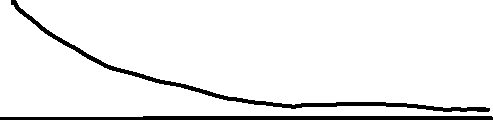
\includegraphics[width=0.3\linewidth]{T4_couterproof.pdf}
    \end{center}

    Выберем $\forall x_0 \in F_1 \implies$ по $T_3$ выберем $\epsilon_{x_0} = \rho(x_0, F_2)/2$
    $U_1 \coloneqq \bigcup_{x_0 \in F_1} B(x_0, \epsilon_{x_0})$.
    $\forall y_0 \in F_2$ выберем $\epsilon_{y_0} = \rho(y_0, F_1)/2$
    $U_2 \coloneqq \bigcup_{y_0 \in F_2} B(y_0, \epsilon_{y_0})$

    $U_1 \supset F_1, U_2 \supset F_2$, $U_1 \cap U_2 = \varnothing$:
    если $z_0 \in U_1 \cap U_2$, то $z_0 \in B(x_0, \epsilon_{x_0}) \cap B(y_0, \epsilon_{y_0})$,
    это значит, что $\rho(x_0, y_0) < \epsilon_{x_0} + \epsilon_{y_0}< 2 \max\{\epsilon_{x_0}, \epsilon_{y_0}\}$.

    Пусть $\epsilon_{y_0} \ge \epsilon_{x_0}$ тогда $\rho(x_0, y_0) < 2 \epsilon_{y_0} = \rho(y_0, F_1)$.
    Получили противоречие.
\end{proof}
\begin{remark}
    Почти верно обратное: если $X$ нормально и $X$ удовлетворяет второй аксиоме счетности, тогда $X$ -- метризуемо.
\end{remark}

\begin{theorem}
    $X$ -- хаусдорфово, тогда $X$ нормально $\Leftrightarrow \forall$ замкнутого $F$,
    $\forall$ открытого $G : G \supset F\ \exists G'$ -- открытое:
    $F \subset G' \subset \Cl G' \subset G$
    (замкнутое $\subset$ открытое $\subset$ замкнутое $\subset$ открытое)
    [так можно делать бесконечно].
\end{theorem}
\begin{proof}
    Это переформулировка нормальности:
    \begin{gather*}
        F \subset G \Leftrightarrow F \cap (X \setminus G) = \varnothing\\
        F \subset G' \subset \Cl G' \subset G\\
        \begin{cases}
            G'\text{ -- окрестность } F \\
            X \setminus \Cl G'\text{ -- окрестность }X \setminus G
        \end{cases}
        \implies G' \cap (X \setminus \Cl G') = \varnothing
    \end{gather*}
\end{proof}

\begin{theorem}
    $X$ компактно + хаусдорфово, тогда $X$ нормально.
\end{theorem}
Напоминание: в $X$ замкнутость равносильна компактности.
\begin{proof}
    $F_1, F_2$ -- замкнуты, $F_1 \cap F_2 = \varnothing$.
    $\forall x,y : x \in F_1, y \in F_2$ выберем $U_{x,y} \cap V_{x,y} = \varnothing$,
    $x \in U_{x,y}, y \in V_{x,y}$

    Зафиксируем $y$ ,
    $\{U_{x,y}\}_{x \in X}$ -- покрытие $F_1$, значит существует конечное подпокрытие:
    $\exists U_{x_1, y},..., U_{x_n, y}$ -- конечное подпокрытие.
    \[U_y \coloneqq \bigcup_{i=1}^n U_{x_i, y}\]
    окрестность $F_1$, не содержит $y$.
    \[W_y \coloneqq \bigcap_{i=1}^n V_{x_i, y}\]
    окрестность $y: U_y \cap W_y = \varnothing$

    $\{W_y\}_{y \in F_2}$ -- покрытие $F_2$.
    Существуют $y_1, ..., y_m: W_{y_1},..., W_{y_m}$ -- покрытие $F_2$
    \[U_{F_1} \coloneqq \bigcap_{i=1}^m U_y\quad U_{F_2} \coloneqq \bigcup_{i=1}^m W_{y_i}\]
    Допустим $z \in U_{F_1} \cap U_{F_2}$
    $\exists i: z \in W_{y_i}$, $z \in U_{y_i}$,
    но $W_{y_i} \cap U_{y_i} = \varnothing$ по построению -- противоречие.
\end{proof}

\begin{theorem}[Урысон]
    $X$ -- нормальное пространство. $F_1, F_2$ -- неперескающиеся замкнутые множества
    $\Leftrightarrow \exists$ непрерывная $f: X \to \R$:
    $f|_{F_1} = 0, f|_{F_2} = 1$ (функциональная отделимость).
\end{theorem}

\textbf{Схема доказательства:}
Обратно: $f: X \to \R$ -- непрерывная: $f|_{F_1} = 0, f|_{F_2} = 1$
\[U_{F_1} \coloneqq f^{-1}((-\infty, 1/2)) \quad U_{F_2} \coloneqq f^{-1}((1/2, +\infty))\]

Прямо: $X$ нормально, $F_0 \cap F_1 = \varnothing$, значит
$G_1 \coloneqq X \setminus F_1, F_0 \subset G_1$
\begin{gather*}
    \implies \exists G_{1/2}: F_0 \subset G_{1/2} \subset \Cl G_{1/2} \subset G_0\\
    \implies \exists G_{1/4}, G_{3/4} \qquad F_i \coloneqq \Cl G_i\\
    F_0 \subset G_{1/4} \subset F_{1/4} \subset G_{1/2} \subset F_{1/2} \subset G_{3/4} \subset F_{3/4} \subset G_1
\end{gather*}
и так далее
Получаем $G_{k/2^n}$ и $F_{k/2^n} \coloneqq \Cl G_{k/2^n}$.
Если $k_1/2^{n_1} < k_2/2^{n_2}$, тогда $G_{k_1/2^{n_1}} \subset F_{k_1/2^{n_1}} \subset G_{k_2/2^{n_2}} \subset F_{k_2/2^{n_2}}$.

Рассмотрим $f(x) \coloneqq \inf\{\alpha: x \in F_\alpha\}$.
Если $x \in F_0 \implies f(x) = 0$, если $x \in F_1 \implies f(x) = 1$.
В качестве упражнения надо доказать непрерывность $f$, тогда $f$ -- искомая функция.
\end{document}